\uuid{frxJ}
\exo7id{5460}
\titre{exo7 5460}
\auteur{rouget}
\organisation{exo7}
\datecreate{2010-07-10}
\isIndication{false}
\isCorrection{true}
\chapitre{Intégration}
\sousChapitre{Intégrale de Riemann dépendant d'un paramètre}
\module{Analyse}
\niveau{L2}
\difficulte{}

\contenu{
\texte{
Etude complète de $F(x)=\int_{x}^{2x}\frac{dt}{\sqrt{t^4+t^2+1}}$.
}
\reponse{
Pour $t\in\Rr$, posons $g(t)=\frac{1}{\sqrt{t^4+t^2+1}}$. $g$ est continue sur $\Rr$ et admet donc des primitives sur $\Rr$. Soit $G$ une primitive de $g$ sur $\Rr$.

\textbf{Définition, dérivabilté, dérivée.}

Puisque $g$ est continue sur $\Rr$, $F$ est définie sur $\Rr$ et pour tout réel $x$, $F(x)=G(2x)-G(x)$. $G$ est de classe $C^1$ sur $\Rr$ et donc $F$ est de classe $C^1$ sur $\Rr$ et pour tout réel $x$,

$$F'(x)=2G'(2x)-G'(x)=2g(2x)-g(x)=\frac{2}{\sqrt{16x^4-4x^2+1}}-\frac{1}{\sqrt{x^4+x^2+1}}.$$

\textbf{Parité.}

Soit $x\in\Rr$. En posant $t=-u$ et donc $dt=-du$, on obtient, en notant que $g$ est paire

$$F(-x)=\int_{-x}^{-2x}g(t)\;dt=\int_{x}^{2x}g(-u).-du=-\int_{x}^{2x}g(u)\;du=-F(x).$$

$F$ est donc impaire.

\textbf{Variations.}

Pour $x$ réel,

\begin{align*}\ensuremath
\mbox{sgn}(F'(x))&=\mbox{sgn}(\frac{2}{\sqrt{16x^4-4x^2+1}}-\frac{1}{\sqrt{x^4+x^2+1}})=\mbox{sgn}(2\sqrt{x^4+x^2+1}-\sqrt{16x^4-4x^2+1})\\
 &=\mbox{sgn}(4(x^4+x^2+1)-(16x^4+4x^2+1))\;(\mbox{par croissance de}\;t\mapsto t^2\;\mbox{sur}\;\Rr^+)\\
  &=\mbox{sgn}(-12x^4+3)=\mbox{sgn}(1-4x^4)=\mbox{sgn}(1-2x^2).
\end{align*}

$F$ est donc strictement croissante sur $[-\frac{1}{\sqrt{2}},\frac{1}{\sqrt{2}}]$ et strictement décroissante sur $]-\infty,-\frac{1}{\sqrt{2}}]$ et sur $[\frac{1}{\sqrt{2}},+\infty[$.

\textbf{Etude en} $\bf{+{\infty}}$.

Pour $x>0$, $0\leq F(x)\leq\int_{x}^{2x}\frac{1}{\sqrt{x^4}}\;dt=\frac{2x-x}{x^2}=\frac{1}{x}$. Comme $\frac{1}{x}$ tend vers $0$ quand $x$ tend vers $+\infty$, le théorème des gendarmes permet d'affirmer que $\lim_{x\rightarrow +\infty}F(x)=0$.

\textbf{Graphe.}

$$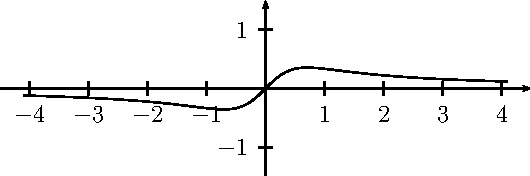
\includegraphics{../images/pdf/frxJ-1.pdf}$$
}
}
